\documentclass{article}
\usepackage{graphicx}
\usepackage{subcaption}
\usepackage{tikz}
\usepackage{fancyhdr}
\usepackage[headheight=30pt, top=1in, bottom=1in]{geometry}
\usepackage[backend=biber]{biblatex}

\title{Research Proposal:\\Surface Analysis of Used Mechanical Heart Valves\\for Microcracks and Defects Detection}
\author{Defne Korkmaz\thanks{RWTH Aachen University} \and Priv.-Doz. Dr. Steffen Brinckmann\thanks{Jülich Forschungszentrum}}
\date{\today}

\addbibresource{reflist.bib}

\pagestyle{fancy}
\fancyhf{} % Clear all header/footer content
\fancyhead[C]{
\includegraphics[width=0.2\textwidth]{rwthlogo.png}\hfill
\includegraphics[width=0.2\textwidth]{jülichlogo.png}}
\renewcommand{\headrulewidth}{1pt}
\fancyfoot[C]{\thepage} % Page number in the center
\renewcommand{\footrulewidth}{1pt}

\begin{document}
\maketitle
\vfill

\pagebreak
\section{Introduction}
*add intro*

\section{Motivation}
My suggested research on "Surface Analysis of Used Mechanical Heart Valves for Microcracks and Defects Detection" seeks to observe the changes in surface quality over the years in valves that were removed. My motivation and intrigue regarding the extent of surface defects on used heart valves and the probable link between service life and valve depreciation stem from studying mechanical engineering for my bachelor's, studying materials engineering for my master's, and also from having a cardiologist father. This study integrates materials engineering and medical ideas and gives insight into the relationship between service duration and surface defects in removed mechanical heart valves. It is expected that the surface quality clearly worsens over the duration of usage. In the later stages of the research, perhaps at the Master’s Thesis stage, an attempt to categorize and/or quantify the surface defects with a machine learning algorithm could be made.





\section{Background and Literature Review}
\subsection*{Heart Valves}
add things here
\subsection*{Related Research}

A relatively old research article regarding the surface analysis of used mechanical heart valves is available. This article revolves around a sample size of 17 heart valves.
\cite*{barmada1998}


\cite*{bjork1971}


\cite*{hutchison2011}


\cite*{venkatesh2013}


\cite*{vansteenbergen2019}


\cite*{wu2001}


\cite*{zhang1995}

\pagebreak

\section{Research Objectives}
\begin{enumerate}
    \item Conduct literature search
    \item Acquire sterilized samples
    \item Prepare the samples, remove suture rings or any extra components
    \item Initial analysis under an optical microscope
    \item Cut and polish the samples
    \item Analyze under an optical microscope
    \item Document findings, collect images
    \item Discuss if there is a correlation between the service life and the amount and extent of surface defects on the valves
    \item Report findings
\end{enumerate}

\section{Sample Collection and Preparation}
Two samples have already been acquired, and the brand and service life of these samples are summarized in the table below.

\begin{center}
    \begin{tabular}{|c|c|c|c|}
        \hline
        Sample & Brand & Material & Service Life \\
        \hline
        1 & Medtronic\cite*{medtronic_image} & Carbon coated titanium & 4 days \\
        \hline
        2 & Björk-Shiley\cite*{björk1969} & Carbon coated titanium & 35 years \\
        \hline
    \end{tabular}
\end{center}

Approximately 10 more samples will be acquired. These samples are expected to have service lives distributed evenly in the range from 1 year to 40 years.
The servie duration of the valves will be noted and each valve will be photographed and labelled.
If necessary, other information regarding the removed heart valves may be collected.



\section{Timeline and Work Plan}
Below is a timeline showing all the past and future milestones of this proposed study.\\

Progress to be made in 2023:
\begin{figure}[h]
    \centering
    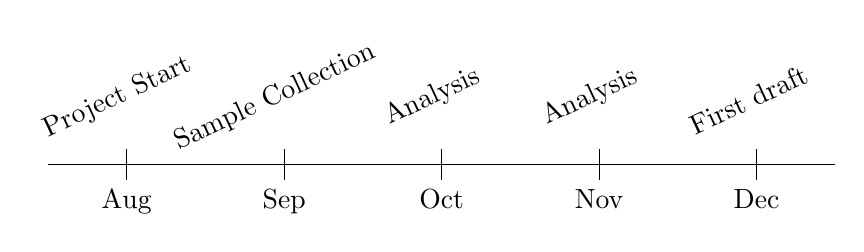
\begin{tikzpicture}
        \draw (0,0) -- (10,0);
        \foreach \x/\month/\labeltext in {1/Aug/Project Start, 3/Sep/Sample Collection, 5/Oct/Analysis, 7/Nov/Analysis, 9/Dec/First draft} {
            \draw (\x,0.2) -- (\x,-0.2) node[below] {\month};
            \node[above, rotate=25] at (\x,0.6) {\labeltext};
        }
    \end{tikzpicture}
    \caption{Project Timeline}
\end{figure}


\section{Ethical Considerations}
The proposed research does not entail any significant ethical considerations. The focus of the study is solely on the material analysis of used replacement heart valves and these valves are obtained anonymously, without any personal or sensitive data linked to the former owners of these implants. Only medical information related to these implants are the following: the brand and model of the implant, and the time spent in the patient's body. Nonetheless, adherence to scientific integrity will always be a priority throughout the research.


\section{Conclusion}
This research proposal outlines the plan to study the surface of used mechanical heart valves for defects. Following a timeline, it is aimed to achieve the goals through research, sample collection, and analysis in a systematic manner.

It is aimed to provide insights into heart valve performance, contributing to a better understanding of the incidence of surface defects on mechanical heart valves. This will help with understanding the most defect-prone regions of the heart valves and ultimately suggest possible improvements.


\pagebreak
\printbibliography
\end{document}
